\chapter{METODOLOGI}
\label{chap:desainimplementasi}

% Ubah bagian-bagian berikut dengan isi dari desain dan implementasi

Metodologi berisi tentang langkah-langkah yang dilakukan untuk mencapai tujuan dari tugas akhir ini, yang dimana langkah-langkah tersebut digambar dalam blok diagram. Secara umum, gambaran blok diagram metodologi yang digunakan dalam pengerjaan tugas akhir ini adalah sebagai berikut. 

\begin{figure} [ht]
  \centering
  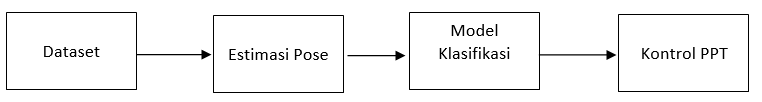
\includegraphics[scale=0.95]{gambar/metodologi.png}
  \caption{Blok Diagram Metodologi}
  \label{fig:Metodologi}
\end{figure}

\section{Dataset}
\label{sec:dataset}

Input citra digunakan sebagai dataset yang nantinya digunakan dalam proses training data. Untuk proses pengambilan dataset dimulai dengan Input citra video. Proses pengambilannya melalui kamera \emph{webcam}, dengan cara mengambil video dan membuatnya menjadi potongan frame-frame. Video yang diambil disesuaikan dengan kelas apa yang ingin diperagakan. Misalnya untuk perintah seperti pengguna \emph{"tool pen"} maka kita harus memperagakan pose \emph{pen} yang telah ditentukan sebelumnya didepan kamera. 

Cara memperagakannya adalah dengan mengambilnya dari beberapa jarak dari dengan kamera. Supaya nantinya deteksi perintah ini dapat terbaca dari berbagai sisi jarak kamera juga. Selain jarak juga dilakukan variasi bentuk pose tangan dan pengambilan angle dibandingkan dengan kamera. Karena, satu orang dalam memeragakan pose tangan tidak selalu sama persis bentuknya dengan yang orang lainnya. 

\begin{longtable}{|c|c|c|}
  \caption{Hasil Pengambilan Dataset}
  \label{tb:Hasil Pengambilan Dataset}\\
  \hline
  \textbf{No.} & \textbf{Kelas Dataset} & \textbf{Citra Dataset} \\
  \hline
  \endhead
  1 & Dataset \emph{Next Slide}  &  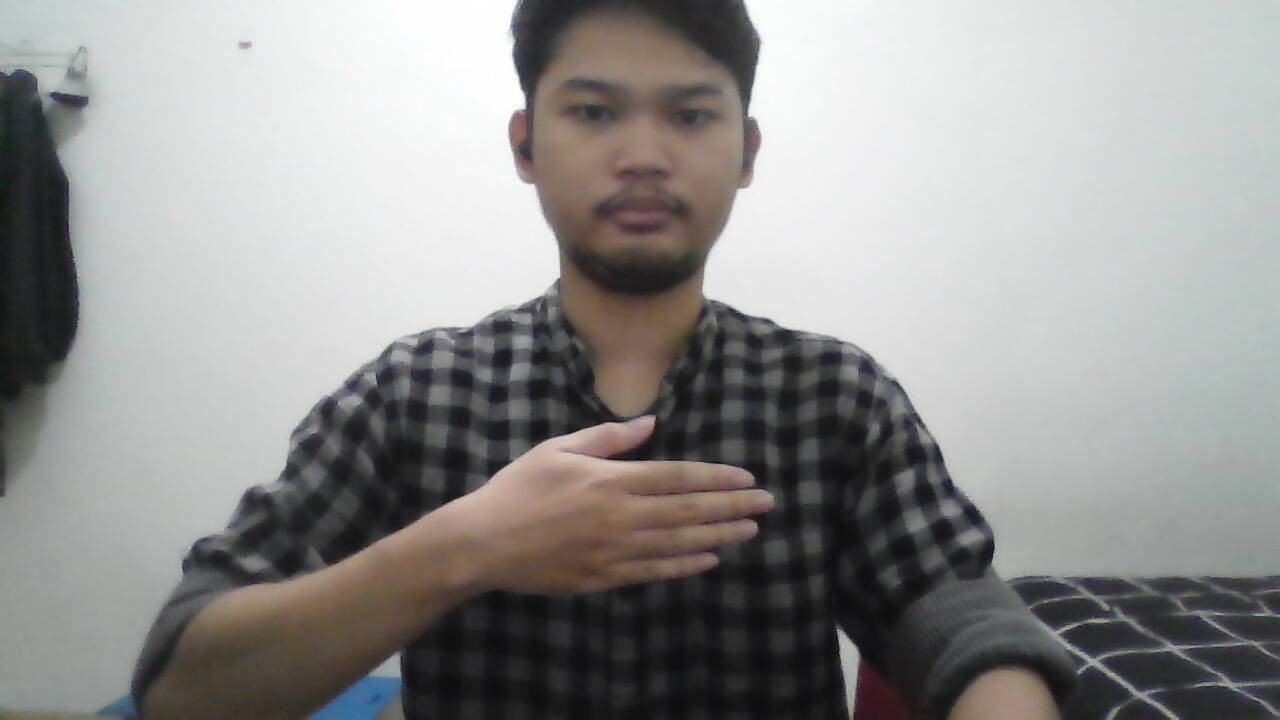
\includegraphics[scale=0.2]{gambar/pengambilan-dataset/dataset-next-slide.jpg} \\
  \hline
  2 & Dataset \emph{Previous Slide}  &  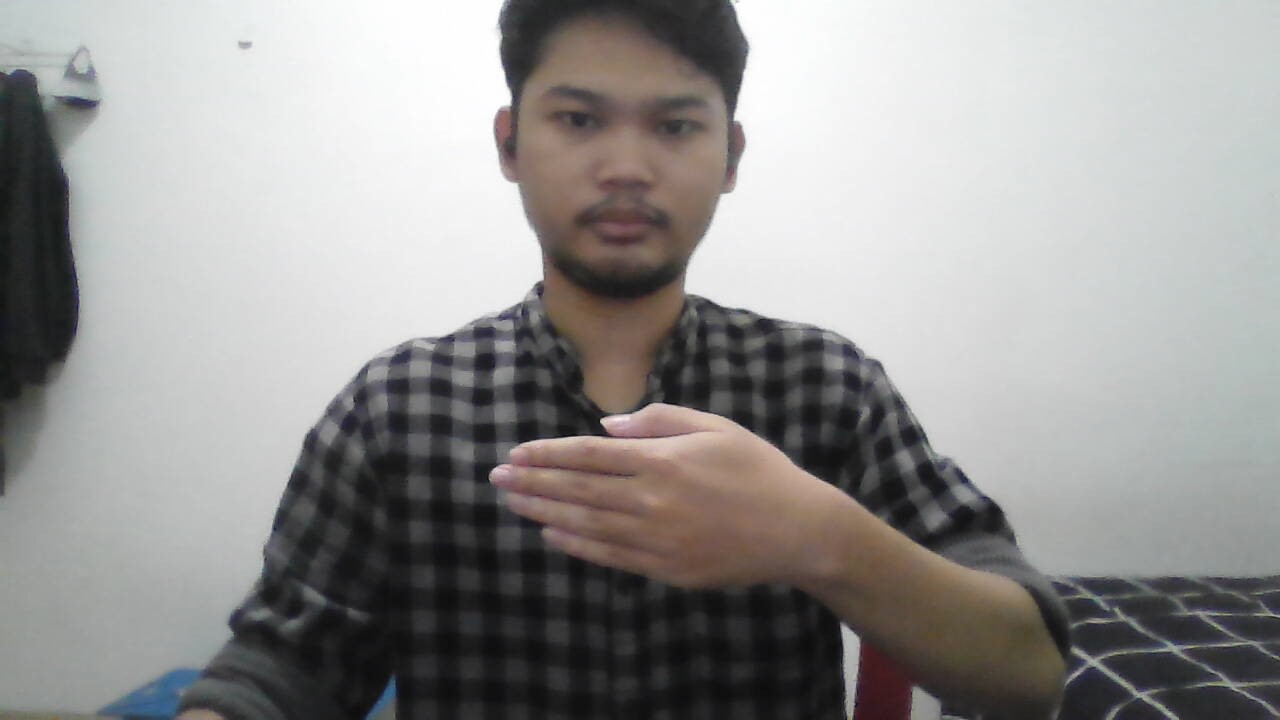
\includegraphics[scale=0.2]{gambar/pengambilan-dataset/dataset-previous-slide.jpg} \\
  \hline
  3 & Dataset \emph{Pointer}  &  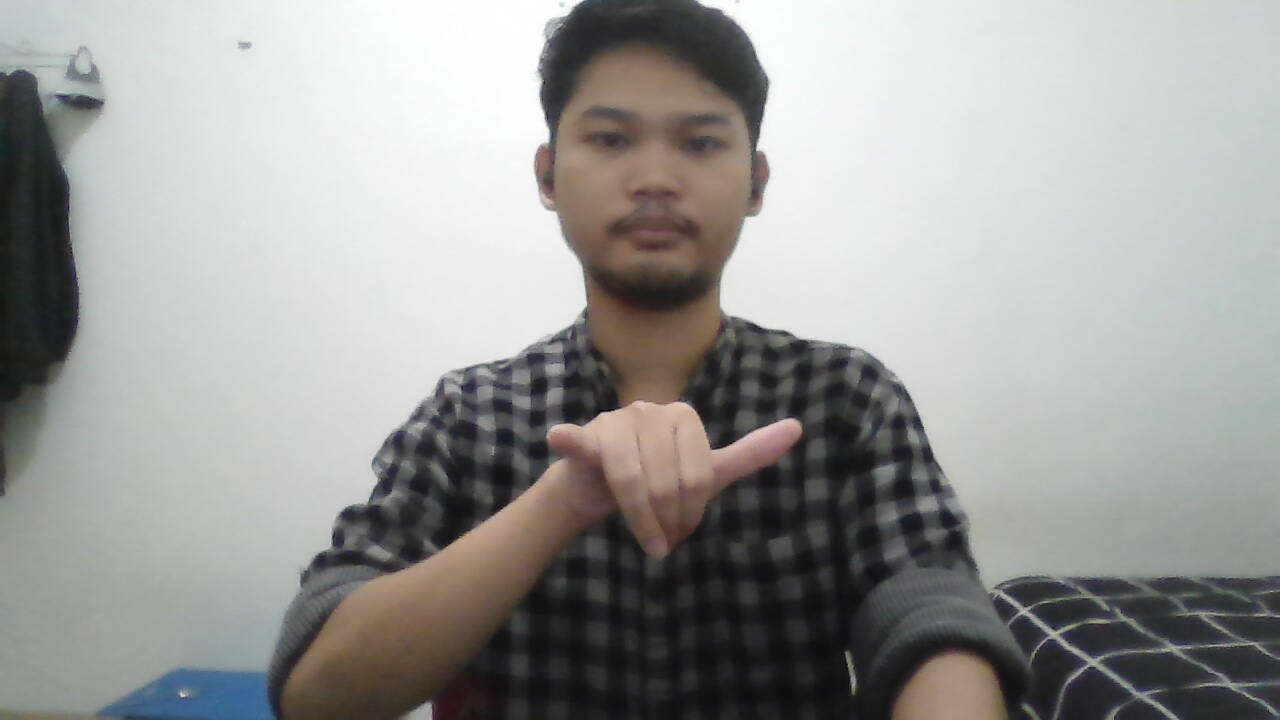
\includegraphics[scale=0.2]{gambar/pengambilan-dataset/dataset-pointer.jpg} \\
  \hline
  4 & Dataset \emph{Zoom Left}  &  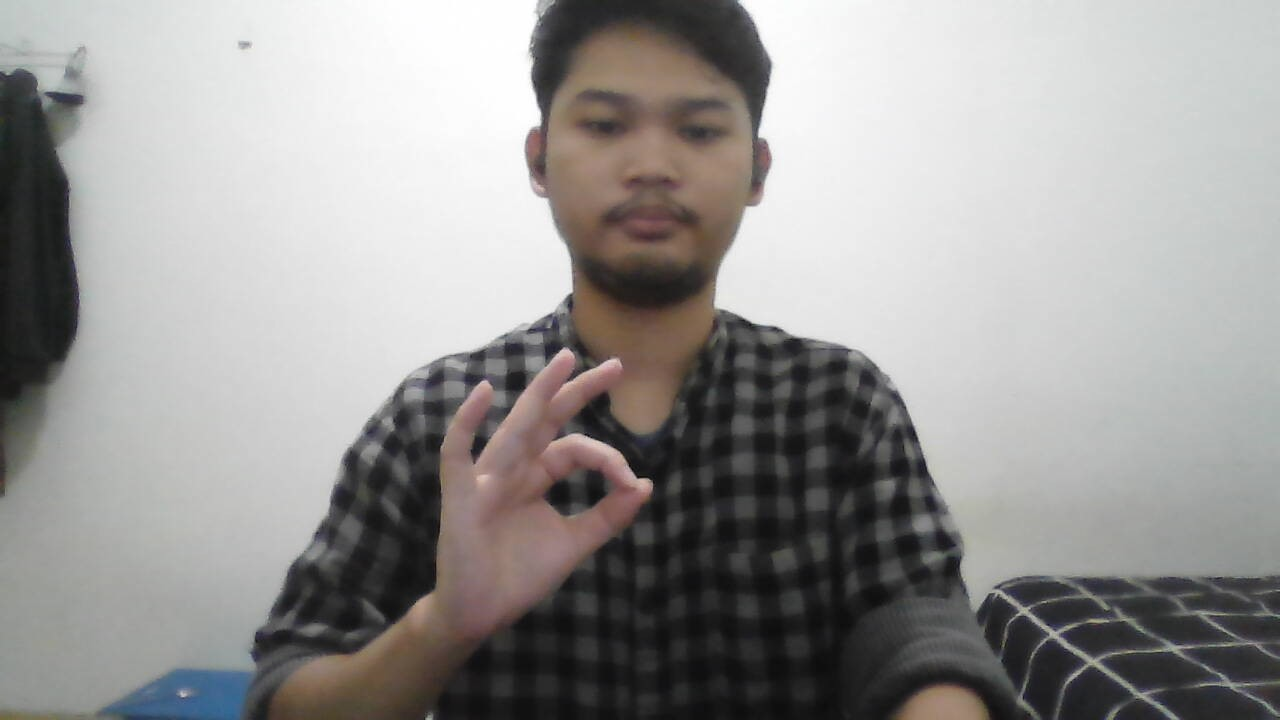
\includegraphics[scale=0.2]{gambar/pengambilan-dataset/dataset-zoom-left.jpg} \\
  \hline
  5 & Dataset \emph{Zoom Right}  &  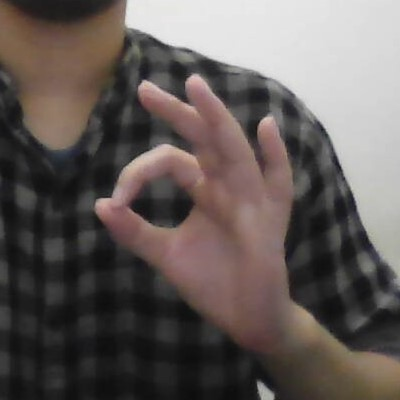
\includegraphics[scale=0.2]{gambar/pengambilan-dataset/dataset-zoom-right.jpg} \\
  \hline
  6 & Dataset \emph{Pen Left}  &  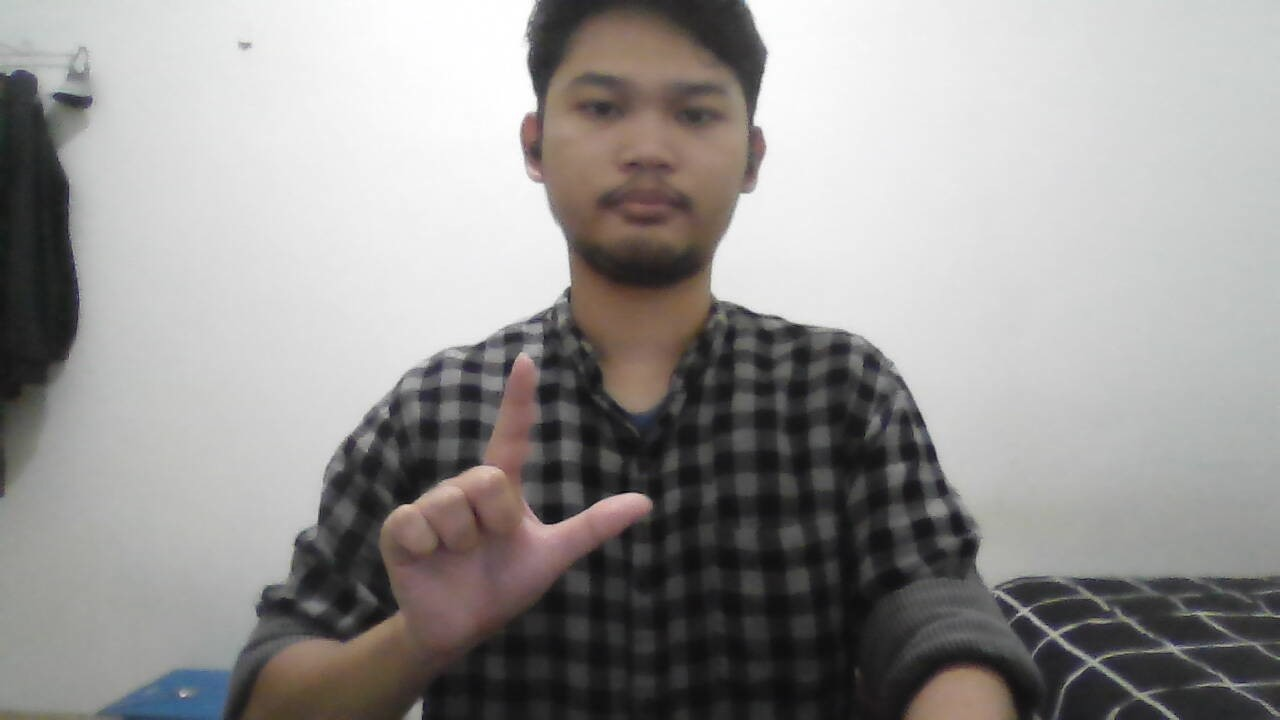
\includegraphics[scale=0.2]{gambar/pengambilan-dataset/dataset-pen-left.jpg} \\
  \hline
  7 & Dataset \emph{Pen Right}  &  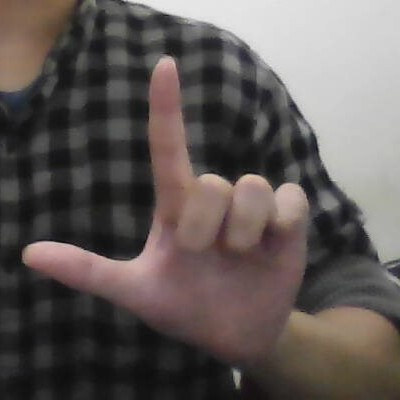
\includegraphics[scale=0.2]{gambar/pengambilan-dataset/dataset-pen-right.jpg} \\
  \hline
  8 & Dataset \emph{Erase}  &  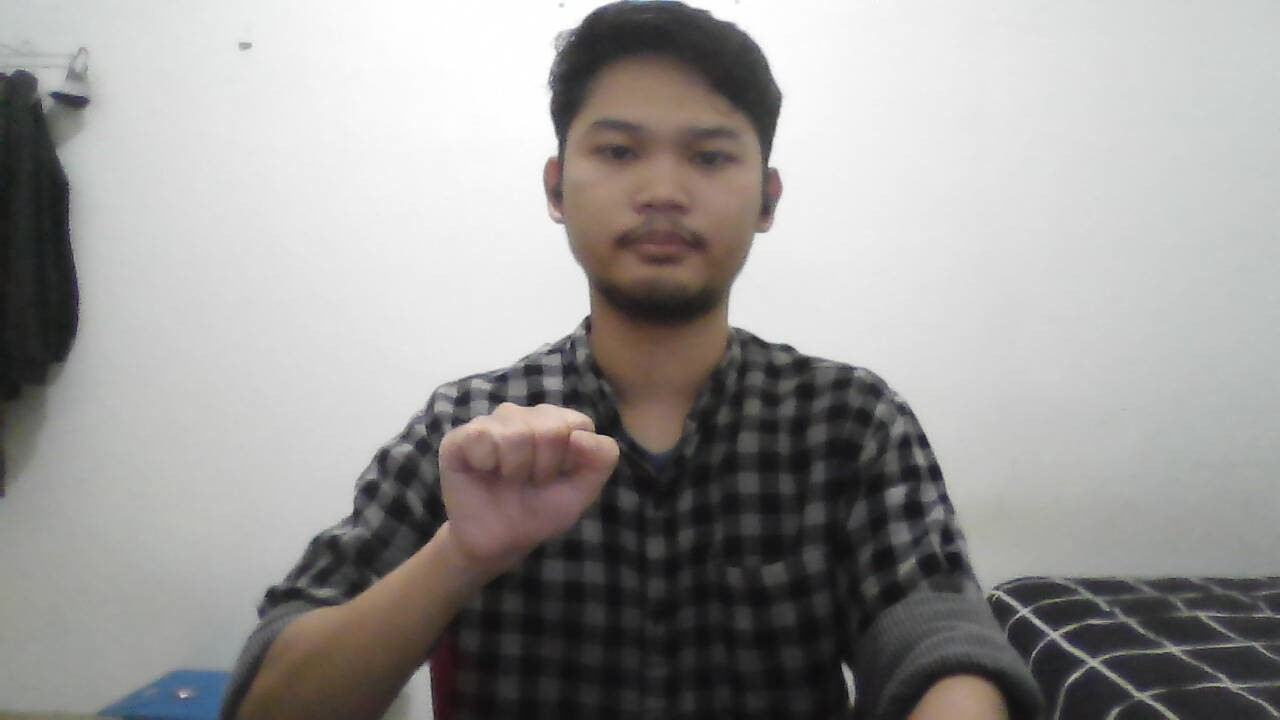
\includegraphics[scale=0.2]{gambar/pengambilan-dataset/dataset-erase.jpg} \\
  \hline
\end{longtable}

Jumlah dan kualitas dari dataset ini juga perlu diperhatikan, karena sangat mempengaruhi kinerja atau hasil tingkat akurasi model yang didapat. Dalam tugas akhir ini banyak citra yang digunakan sebanyak 300 citra pada masing-masing kelas. Karena kelas yang dibuat terdapat delapan kelas, maka total banyaknya citra yang digunakan adalah 2400 citra. Hasil dari pengambilan dataset beserta bentuk pose tangan tiap kelasnya, dapat dilihat dalam Tabel \ref{tb:Hasil Pengambilan Dataset}.

Pada prinsipnya, semakin banyak data akan menambah tingkat akurasi dari sebuah model. Namun, belum ditemukan satu aturan khusus yang pasti mengenai jumlah batas minimal data yang dibutuhkan untuk melatih model dengan tingkat hasil akurasi tertentu. Jumlah data tersebut bergantung pada masalah yang diselesaikan \parencite{Junghwan}. Oleh karenanya, penentuan berapa banyak jumlah data ini perlu dilihat pula hasil akurasinya. Apabila akurasi dirasa cukup maka jumlah dataset tersebut dapat dinyatakan cukup.

Dalam Tabel \ref{tb:Hasil Pengambilan Dataset}, bisa dilihat bahwa pose yang dibuat berjumlah delapan. Padahal banyaknya fungsi yang ingin diterapkan berjumlah enam (\emph{next slide, previous slide, pointer, zoom, pen,} dan \emph{erase}). Hal ini dilakukan karena model yang dibuat, diharapkan dapat mendeteksi tidak hanya menggunakan salah satu tangan saja. Namun, bisa digunakan baik menggunakan tangan kanan maupun tangan kiri. 

Tetapi, tidak semua pose perlu dataset dengan citra dari tangan kanan dan kiri. Karena beberapa pose memiliki kemiripan antara bentuk tangan kanan dan kiri. Dapat dilihat dalam Tabel \ref{tb:Hasil Pengambilan Dataset} bahwa pose untuk fungsi \emph{next slide, previous slide, pointer,} dan \emph{erase} hanya memiliki masing-masing satu kelas. Apabila dilakukan \emph{mirroring} pada citra tersebut hasilnya juga tidak jauh beda. Sehingga, model masih bisa mendeteksi.

Namun, untuk fungsi \emph{pen} dan \emph{zoom} diperlakukan berbeda. Karena bentuk posenya apabila dibandingkan antara menggunakan tangan kanan dengan tangan kiri, terlihat perbedaan yang cukup jauh. Oleh karena itu, cara termudah untuk model dapat mendeteksi tangan kanan maupun kiri dalam pose \emph{pen} dan \emph{zoom} adalah dengan memisahnya menjadi kelas dataset yang terpisah. Hal ini lah yang membuat jumlah kelas dataset terdapat delapan, walaupun jumlah fungsi kontrol \emph{Power Point} yang ingin diterapkan hanya berjumlah enam.

Ukuran frame yang terlihat pada Tabel \ref{tb:Hasil Pengambilan Dataset} sendiri, perlu dipotong supaya hanya citra dari pose tangannya saja yang ditangkap. Namun, proses ini baru bisa dilakukan jika sudah dapat mendeteksi posisi tangan yaitu pada bagian proses estimasi pose. Citra yang digunakan input merupakan citra berwarna yang memiliki tiga buah kanal warna. Tiga buah kanal ini terdiri dari komponen warna RGB yaitu merah/\emph{Red} (R), green/\emph{Green} (G), dan biru/\emph{Biru} (B) yang memiliki nilai dengan rentang mulai dari 0 sampai 255 \parencite{PriyantoHidayatullah}. 

Sebuah dataset perlu dibagi menjadi dua bagian yaitu training set dan validation set. Pembagian ini diperlukan agar dapat mencegah overfitting dan untuk mengevaluasi model. Overfitting yang dimaksud disini adalah kondisi yang terjadi saat model memiliki performa yang sangat baik namun hanya terjadi untuk dataset pelatihan saja. Apabila model diberi data yang belum pernah dilihat sebelumnya, maka performa yang dihasilkan menjadi buruk.

Sebagian besar data dari dataset merupakan Training set. Hal ini karena data pada training set digunakan untuk pelatihan. Apabila proses pelatihan ini selesai, dilakukan proses evaluasi kinerja dari model menggunakan data dari validation set. Jumlah, pembagian banyaknya data pada trainining set dan validation set dalam tugas akhir ini adalah 75\% : 25\%. Proses pengambilan training set dan validation set juga terpisah. Karena model idealnya tidak boleh dilatih menggunakan sample pada validation set, baik sebagian maupun seluruhnya. Sehingga antar training set dan validation set berisi data yang sepenuhnya berbeda. 

\section{Estimasi Pose}
\label{sec:poseprediction}

Estimasi pose memproses frame yang didapat dari hasil pengambilan dataset sebelumnya. Proses ini berguna untuk menentukan \emph{keypoint} untuk membuat kerangka dari pose tangan atau yang disebut \emph{landmark}. Citra tangan dari input kamera yang masih asli, diekstrak menjadi citra yang sudah terdapat kerangka posenya sehingga dapat dianalisa untuk melakukan pengklasifikasian. Dalam proses pendeteksian pose kerangka tangan, penulis menggunakan bantuan sebuah \emph{library} bernama \emph{mediapipe}. \emph{MediaPipe Hands} menggunakan \emph{machine learning} untuk menemukan 21 \emph{landmark} 3D tangan hanya dari satu frame. Tiap frame ini diproses lagi ketahapan selanjutnya bernama ekstraksi fitur. 

Ekstraksi fitur merupakan bagian dari tahapan yang untuk pengenalan pola. Proses ini dilakukan agar dapat memperoleh informasi yang terkandung dalam suatu citra. Jika informasi ini telah didapatkan, maka informasi tersebut digunakan sebagai acuan untuk membedakan antara satu citra dengan citra yang lainnya. Ektraksi fitur ini dapat dilakukan, salah satunya dengan cara memisahkan antara objek dengan \emph{background}. Dalam hal ini, deteksi \emph{landmark} tangan dipisah dari \emph{background} aslinya dan diganti dengan latar berwarna hitam. Sehingga, hanya menyisakan citra berupa \emph{landmark} dari pose tangan saja tanpa ada citra tangan yang asli.   

Hasil dari ekstraksi fitur tersebut, diproses lagi dengan proses \emph{localization}. Proses ini menentukan lokasi objek dengan membuat kotak pembatas pada daerah citra yang terdapat pose tangannya. Kotak pembatas inilah yang menentukan seberapa besar bagian citra yang dipotong. Apabila gambar sudah diganti dengan \emph{background} hitam, selanjutnya gambar dikumpulkan perkelas untuk dijadikan input proses \emph{training}.

Berdasarkan proses \emph{localization} yang dilakuakan, citra dipotong menjadi ukuran frame sebesar 128 x 128 piksel dengan posisi menyesuaikan letak \emph{landmark} tangan. Diberikan juga \emph{padding} sebesar 64 dikiri, atas, kanan, dan bawah citra. Tujuannya agar tidak ada informasi dari ujung-ujung \emph{landmark} yang hilang karena terpotong. Hasilnya seperti yang terlihat pada gambar \ref{tb:Hasil Estimasi Pose}. Hasil dari proses ini kemudian disimpan lagi dalam folder sesuai dengan kelas dari pose yang dilakukan.

\begin{longtable}{|c|c|c|}
  \caption{Hasil Estimasi Pose}
  \label{tb:Hasil Estimasi Pose}\\
  \hline
  \textbf{No.} & \textbf{Kelas Pose} & \textbf{Hasil Citra Estimasi Pose} \\
  \hline
  \endhead
  1 & \emph{Next Slide}  &  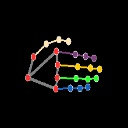
\includegraphics[scale=0.85]{gambar/pose_prediction_next_slide.jpg} \\
  \hline
  2 & \emph{Previous Slide}  &  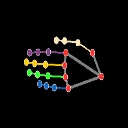
\includegraphics[scale=0.85]{gambar/pose_prediction_previous_slide.jpg} \\
  \hline
  3 & \emph{Pointer}  &  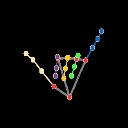
\includegraphics[scale=0.85]{gambar/pose_prediction_pointer.jpg} \\
  \hline
  4 & \emph{Zoom Left}  &  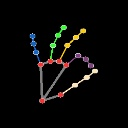
\includegraphics[scale=0.85]{gambar/pose_prediction_zoom_left.jpg} \\
  \hline
  5 & \emph{Zoom Right}  &  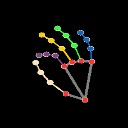
\includegraphics[scale=0.85]{gambar/pose_prediction_zoom_right.jpg} \\
  \hline
  6 & \emph{Pen Left}  &  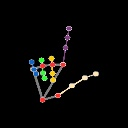
\includegraphics[scale=0.85]{gambar/pose_prediction_pen_left.jpg} \\
  \hline
  7 & \emph{Pen Right}  &  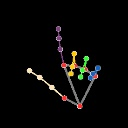
\includegraphics[scale=0.85]{gambar/pose_prediction_pen_right.jpg} \\
  \hline
  8 & \emph{Erase}  &  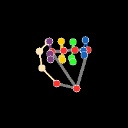
\includegraphics[scale=0.85]{gambar/pose_prediction_erase.jpg} \\
  \hline
\end{longtable}

\section{Model Klasifikasi}
\label{sec:modelklasifikasi}

Tujuan dari pembuatan model adalah dapat menghasilkan model klasifikasi yang dapat memberikan \emph{output} berupa hasil deteksi berdasarkan citra yang diinputkan. Berikut ini proses pembuatan model serta cara memprediksinya. 

\subsection{Pembuatan Model}

Proses pembuatan model dicapai dengan mengatur layer serta \emph{hyperparameter}-nya. Umumnya pengaturan layer ini dibagi menjadi tiga bagian yaitu \emph{convolution layer, pooling layer,} dan \emph{fully connected layer}. Dalam pembuatannya tipe model yang digunakan adalah \emph{Sequential. Sequential} merupakan salah satu cara membuat model dalam \emph{Keras}. Cara ini membuat model dapat dibangun dari satu \emph{layer} ke\emph{layer} lainnya.

Gambaran arsitektur layer model CNN yang digunakan dapat dilihat pada Gambar \ref{fig:cnnlayer}. \emph{Stride} atau jarak perpindahan konvolusi pada semua layer konvolusi sama yaitu satu. Artinya, filter bergeser sebesar satu kotak ukuran matriks pada setiap operasinya. Padding yang digunakan pada semua layer konvolusi dimodel ini juga sama, yaitu valid padding. Valid padding berarti tanpa menggunakan padding sama sekali. Sehingga, output yang dihasilkan (bisa disebut juga dengan \emph{feature map}) berkurang ukurannya masing-masing satu pada kiri, kanan, atas, dan bawah. Jadi, jika ukuran input citranya 128 x 128 maka setelah dikonvolusi hasilnya menjadi 126 x 126. Ukuran filter atau kernelnya yang digunakan tiap konvolusi layer dalam model ini sendiri sama yaitu berukuran 3 x 3. Pada layer pertama jumlah filter yang digunakan sebesar 32. 

\begin{figure} [ht]
  \centering
  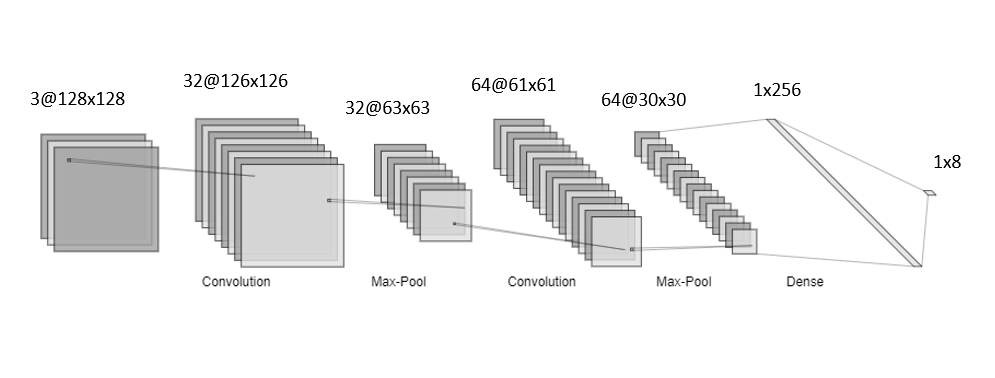
\includegraphics[scale=0.75]{gambar/cnn-layer.png}
  \caption{CNN Layer}
  \label{fig:cnnlayer}
\end{figure}

Pada layer kedua, dilakukan proses \emph{max pooling}. Ukuran max pooling yang digunakan sebesar 2 x 2. Karena ukuran yang digunakan 2 x 2, maka hasil dari pooling layer ini menghasilkan matriks dengan ukuran sebesar setengah dari sebelumnya. Apabila layer yang dilakukan pooling awalnya sebesar 126 x 126, maka hasil setelah dilakukan pooling adalah sebesar 63 x 63.

Dalam layer ketiga, dilakukan proses konvolusi lagi. \emph{Stride}, ukuran filter dan padding yang digunakan sama dengan layer pertama, yang membedakan hanya pada jumlah filternya yang sebesar 64 filter. Layer keempat dilakukan pooling lagi dengan pengaturan sama persis dengan pooling pada layer kedua. Hasilnya berupa feature map berukuran 30 x 30.

Feature map yang dihasilkan dari ekstraksi fitur perlu melakukan flatten karena masih berbentuk multidimensional array. Dari proses tersebut didapatkan sebuah vector. Hal ini bertujuan agar bisa digunakan sebagai input dari fully-connected layer. Lapisan Fully-connected adalah lapisan dimana semua neuron aktivitas dari lapisan sebelumnya terhubung semua dengan neuron di lapisan selanjutnya. Lapisan ini digunakan dengan tujuan untuk mengolah data sehingga bisa diklasifikasikan nantinya. Oleh karena itu, pada Gambar \ref{fig:cnnlayer} bagian paling kanan adalah hasil akhir dimana terdapat array berukuran 1 x 8. Dimana, angka delapan ini menunjukkan jumlah kelas yang ada dalam model ini.

Selain dilakukan pengaturan layer-layer yang digunakan, terdapat hyperparameter yang perlu dikonfigurasi, sebelum melakukan training. Seperti misalnya adalah jumlah epochs, yang digunakan. Epochs sendiri adalah hyperparameter yang memiliki fungsi dalam menentukan banyaknya pengulangan dalam menjalankan algoritma learning dalam proses training. Banyaknya epochs yang digunakan dalam model ini adalah 20 epochs. 

% Proses training ini dimulai dari operasi konvolusi matriks citra, yang kemudian dilanjutkan dengan proses \emph{Max Pooling}. Proses ini dijalankan untuk menghasilkan fitur dari citra yang diinputkan.  

% Terdapat beberapa konfigurasi hyperparameter yang perlu dilakukan terlebih dahulu. Adapun konfigurasi hyperparameter yang dilakukan untuk dataset yang di-train yaitu:

% \begin{enumerate}[nolistsep]
%   \item Epochs. Epochs adalah hyperparameter yang berfungsi untuk menentukan jumlah pengulangan atau berapa kali suatu algoritma learning melakukan proses learning suatu dataset training. Secara sederhana, semakin besar jumlah epochs maka model yang dihasilkan memiliki tingkat akurasi yang lebih tinggi namun waktu yang dibutuhkan untuk melakukan learning akan semakin lambat.
%   \item Batch-Size. Batch-size adalah hyperparameter yang berfungsi untuk mengontrol jumlah sampel training untuk dikerjakan sebelum parameter internal model diperbarui
%   \item Image Size. Image size adalah dimensi ukuran citra yang diterapkan pada dataset. Secara sederhana, semakin kecil dimensi ukurang dari suatu citra maka semakin singkat waktu yang dibutuhkan untuk melakukan proses training.
%   \item Learning Rate. Learning rate adalah hyperparameter yang mengontrol seberapa besar perubahan suatu model dalam menanggapi estimasi kesalahan pada tiap kali weight model diperbarui. Pemilihan nilai learning rate yang tepat diperlukan karena
%   ketika nilai learning rate terlalu kecil maka dapat mengakibatkan proses train yang lama, sedangkan jika nilai learning rate terlalu besar maka dapat mengakibatkan proses learning yang kurang optimal dan terlalu cepat atau proses train yang tidak stabil.
%   \item Optimizer. Optimizer merupakan algoritma atau metode yang digunakan untuk meminimisasi eror (loss function) atau untuk memaksimalkan efisiensi dari produksi. Optimizer merupakan fungsi matematis yang bergantung pada parameter model yang dapat dipelajari seperti weight dan biases. Optimizer sangat membantu untuk mengetahui bagaimana cara mengubah weights ataupun learning rate dari suatu neural network untuk mengurangi nilai loss (Musstafa, 2021). Jenis Optimizer diantaranya yaitu: Adam, Gradient Descent, dan Stochastic Gradient Descent (SGD)
%   (Gupta, 2021).
% \end{enumerate}

\subsection{Prediksi Model}
\label{subsec:Prediksi Model}

Fungsi dari prediksi model klasifikasi ini adalah untuk menyatakan suatu objek kedalam kategori yang sudah ditentukan dengan cara membandingkan input kamera dengan hasil training model mana yang sesuai. Bagian awal dari proses ini adalah deteksi objek tangan yang dimana prosesnya sudah ditangani oleh \emph{framework} mediapipe. Apabila objek tangan terdeteksi, dilanjut dengan proses yang namanya \emph{localization}. \emph{localization} menjadi bagian dari klasifikasi yang menambahkan citra dengan menentukan lokasi objek dengan bantuan \emph{bounding box} atau kotak pembatas. 

Tujuan utama deteksi objek adalah memprediksi lokasi objek dengan \emph{bounding box} atau kotak pembatas dan melakukan klasifikasi objek yang ada pada setiap \emph{bounding box}. Input pada deteksi objek adalah citra yang mengandung satu objek tangan. Sedangkan outputnya adalah hasil prediksi lokasi objek dengan \emph{bounding box} dan klasifikasi kelasnya \parencite{MElgendy}. Ukuran dari kotak ini disamakan dengan dataset yang di-\emph{training}, yaitu 128 x 128. Termasuk juga, didalamnya diberikan padding 64 piksel disemua sisinya seperti yang dilakukan pada Subbab \ref{sec:poseprediction}.

Dalam memprediksi pose yang diinputkan melalui kamera, digunakan sebuah fungsi yang ada pada \emph{library keras}. Output dari fungsi ini adalah array dengan jumlah index sebanyak jumlah kelas yang ada pada model. Sehingga, dari hasil array ini dapat dipilih nilai prediksi yang paling memenuhi untuk klasifikas kelas kita. 

Tampilan secara \emph{real time} hasil prediksi pada program seperti terlihat pada gambar \ref{fig:hasilprediksimodelklasifikasi}. Jika input dari kamera mendeteksi ada pose atau gerakan yang sesuai dengan daftar klasifikasi yang ada, maka proses selanjutnya adalah mengimplementasikan hasil klasifikasi tersebut kedalam aplikasi presentasi yang digunakan.

\begin{figure}[ht]
  \centering
  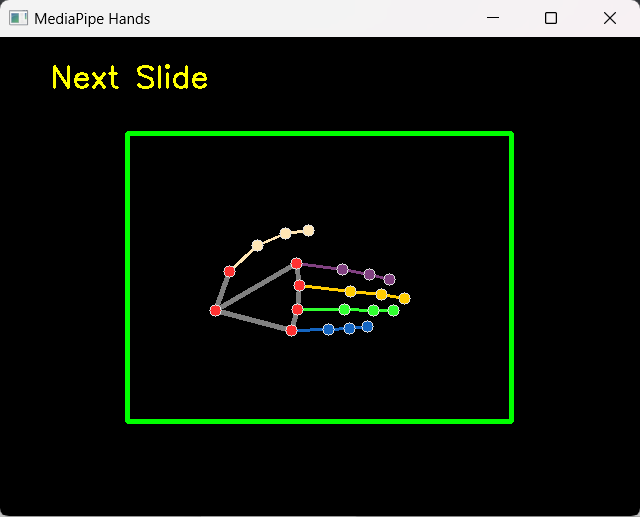
\includegraphics[scale=0.6]{gambar/hasil-prediksi-model-klasifikasi.png}
  \caption{Hasil Prediksi Model Klasifikasi}
  \label{fig:hasilprediksimodelklasifikasi}
\end{figure}

\section{Kontrol PPT}
\label{kontrolppt}

Tahapan ini menghubungkan hasil klasifikasi yang didapatkan dari model, kedalam aplikasi presentasi yang digunakan. Proses implementasi ini membuat program \emph{python} yang dibuat terhubung dengan aplikasi \emph{Microsoft Power Point}. Saat terhubung dilakukan penerapan aksi kontrol kedalam slide presentasi sesuai dengan pose yang terdeteksi.

\subsection{Menghubungkan dengan Fungsi Kontrol PPT}
\label{Menghubungkan dengan Fungsi Kontrol PPT}

Proses ini menggunakan \emph{libray} yang ada pada \emph{python} bernama \emph{pywin32}. Didalamnya terdapat beberapa fungsi yang dapat diakses untuk menavigasi aplikasi \emph{PowerPoint}. Beberapa fungsi dalam aplikasi \emph{Microsoft Power Point} yang dapat diakses adalah seperti navigasi ke slide selanjutnya, navigasi ke slide sebelumnya, dan mengaktifkan \emph{tool pointer}. 

Selain itu, ada cara lain untuk menghubungkan aplikasi \emph{Microsoft Power Point} dengan program yang dibuat yaitu dengan mengakses berbagai macam \emph{shortcut keyboard} yang tersedia. Cara ini dapat dilakukan karena \emph{Microsoft Power Point} memang menyediakan fitur untuk mengontrol presentasi menggunakan keyboard. Sebagai contoh, untuk mengakses fungsi \emph{"pen tool"} dapat menekan tombol \emph{"ctrl"} dan \emph{"p"} secara bersamaan. Daftar lengkap shortcut keyboard untuk kontrol presentasi yang digunakan dalam tugas akhir ini, dapat dilihat pada tabel \ref{tb: daftarshortcutkeyboardmicrosoftpowerpoint}. Perlu diketahui juga, dalam penerapan cara ini dibutuhkan \emph{library pyautogui} supaya dapat mengakses \emph{keyboard} pada perangkat komputer yang digunakan. 

\begin{longtable}{|c|c|}
  \caption{Daftar \emph{Shortcut Keyboard Microsoft Power Point}}
  \label{tb: daftarshortcutkeyboardmicrosoftpowerpoint}\\
  \hline
  \textbf{Perintah Kontrol} & \textbf{Shortcut Keyboard} \\
  \hline
  \emph{erase}   & \emph{'e'}  \\
  \emph{next slide}   & Panah Kanan  \\
  \emph{previous slide}   & Panah Kiri  \\
  \emph{pointer}   & \emph{'ctrl + l'}  \\
  \emph{pen}   & \emph{'ctrl' + 'p'}  \\
  \emph{zoom}   & \emph{'ctrl' + 'mouse wheel up'}  \\
  \hline
\end{longtable}

\subsection{Kontrol Navigasi}
\label{Kontrol Navigasi}
Dalam mengontrol navigasi (\emph{next slide} dan \emph{previous slide}), proses yang dilakukan cukup dengan memanggil fungsi dalam \emph{library pyautogui}. Namun, terdapat satu permasalahan ketika setiap hasil deteksi pose langsung dihubungkan dengan fungsi tersebut. Dimana, aplikasi \emph{Power Point} menjalankan fungsi \emph{next} atau \emph{previous} tersebut secara terus menerus. 

Oleh karena itu, perlu dibuatkan kondisi apabila terdeteksi pose navigasi, maka jalankan fungsi \emph{next} atau \emph{previous} sekali saja. Caranya dengan memberi jeda atau \emph{delay} agar tidak memproses hasil prediksi selanjutnya. Delay yang digunakan adalah sebesar satu detik.

\subsection{Kontrol \emph{Pointer}}
\label{subsec:Kontrol Pointer}

Beberapa perintah tertentu juga perlu menggunakan \emph{cursor} dalam penggunaannya. Salah satunya adalah {tool} untuk \emph{pointer}. Hal ini berarti, dalam penerapannya perlu menghubungkan dengan \emph{library cursor} dan mengubah titik koordinatnya supaya bergerak menyesuaikan gerakan tangan. Oleh karena itu, perlu ditentukan satu titik landmark yang menjadi acuan gerak cursor tersebut. 

Titik landmark yang dipilih adalah titik ke-8, yaitu bagian ujung telunjuk tangan (daftar titik \emph{landmark} dapat dilihat pada Tabel \ref{tb:keterangansetiaptitiklandmark}). Titik ini dipilih karena secara natural dapat menjadi acuan dalam menunjuk sesuatu. Penggunaan ujung telunjuk dapat dirasa lebih memudahkan pengguna untuk menentukan di titik mana pose ingin diarahkan. Penggunaan titik acuan ini juga diterapkan untuk fungsi yang lainnya, yaitu zoom dan pen.

Penghubungan antara input gambar dengan titik koordinat pergerakan \emph{cursor} dilakukan dengan memanfaatkan kemampuan fitur bawaan dari \emph{mediapipe}. Dalam \emph{mediapipe}, dapat diambil data koordinat posisi tangan relatif terhadap ukuran panjang dan lebar kamera. Nilai koordinat yang didapatkan memiliki rentang mulai dari 0 sampai 1. Namun, data ini bersifat \emph{mirror} atau terbalik karena diambil melalui kamera. Jadi, misalnya ukuran kamera yang digunakan adalah 640 x 480. Maka koordinat (0, 0) dalam \emph{mediapipe} berada pada titik piksel (640, 0). Sedangkan untuk koordinat (1, 1), maka letak pikselnya berada pada (0, 480). 

Koordinat yang didapat dari \emph{mediapipe} ini dihubungkan dengan ukuran layar dari komputer, supaya dapat menggerakkan \emph{cursor} pada titik yang diinginkan dalam layar. Cara dalam menghubungkannya melalui operasi perkalian antara rentang koordinat yang didapat dari \emph{mediapipe} dengan ukuran layar. Hasil ini yang menjadi input untuk menentukkan titik \emph{cursor} perlu digerakkan kemana.

Sebagai contoh hasil penerapannya, dapat dilihat pada gambar \ref{fig:Kontrol Pointer}. Dilakukan proses pengaktifan fungsi \emph{pointer} dengan menggunakan hasil klasifikasi pose tangan yang didapatkan dari proses prediksi model yang telah dijelaskan dalam Subbab \ref{subsec:Prediksi Model}.

\begin{figure}[ht]
  \centering
  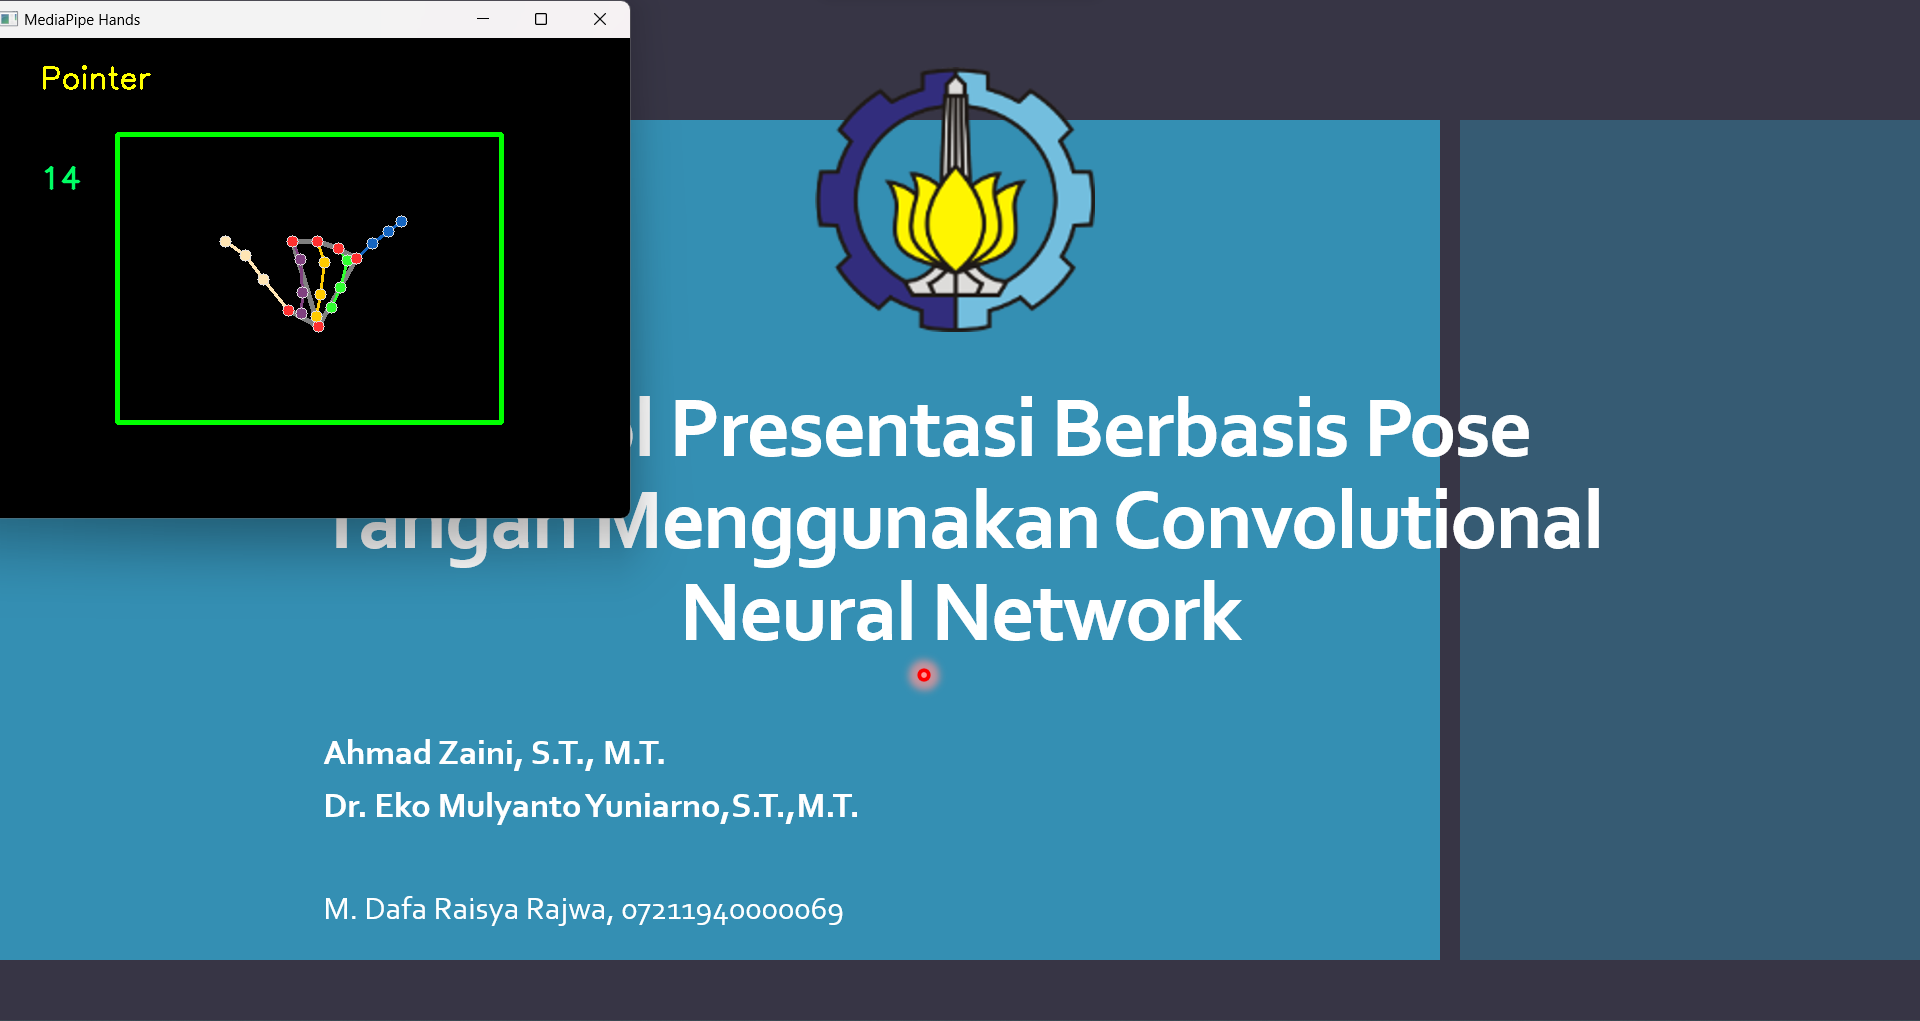
\includegraphics[scale=0.38]{gambar/hasil-kontrol-PPT.png}
  \caption{Kontrol Pointer}
  \label{fig:Kontrol Pointer}
\end{figure}

\subsection{Kontrol \emph{Pen}}
\label{subsec:Kontrol Pen}

Dalam penerapan fungsi \emph{pen} penentuan titik koordinatnya sama persis dengan yang fungsi \emph{pointer} yang dijelaskan pada Subbab \ref{subsec:Kontrol Pointer}. Pembedanya adalah pada kondisi untuk menggambarnya. Pada kontrol ini saat posisi pose \emph{pen} terdeteksi, program dibuat untuk berpindah \emph{state} kedalam mode menggambar.

Perubahan \emph{state} yang dilakukan memiliki tujuan tertentu. Pertama, dapat menghindari perubahan hasil deteksi ketika sedang menggerakkan tangan ketika menggambar. Selain itu, saat berubah \emph{state} proses prediksi model untuk klasifikasi juga tidak dijalankan. Sehingga saat sedang menggambar diharapkan tidak terjadi proses komputasi yang tidak perlu dan bisa menurunkan \emph{frame rate}.

Pada \emph{state pen} ini mengaktifkan fitur \emph{pen} dan menggerakkan \emph{cursor}, namun tidak menekan tombol klik. Penekanan tombol klik baru dilakukan ketika bagian ujung jempol dihubungkan dengan jari tengah. mekanisme tersebut dibuat agar penggunaan fitur \emph{pen} terasa lebih mudah seperti menggunakan \emph{mouse}. Cara kerjanya adalah dengan mengukur jarak antara titik ujung jempol dengan bagian dari jari tengah. Tepatnya pada titik \emph{landmark} ke-10 dan ke-4 (Detail letak titik ini dapat dilihat pada Tabel \ref{tb:keterangansetiaptitiklandmark}). Jika jaraknya diangka lebih kecil dari 0,05 maka program mengirimkan input untuk menekan klik kiri pada \emph{mouse} dan jika tidak maka penekanan klik ini akan dilepaskan.

\subsection{Kontrol \emph{Zoom In}}
\label{subsec:Kontrol Zoom In}

Kontrol zoom pada dasarnya sama dengan pen, yang membedakan pada kondisi \emph{trigger} fungsi zoom. Pada kontrol ini yang menjadi acuan adalah jarak antara ujung jempol dengan ujung telunjuk. Lebih tepatnya titik \emph{landmark} ke-8 dan ke-4. Jika jaraknya masih terhitung menempel maka fungsi zoom belum dijalankan. Namun, jika jaraknya mulai menjauh baru menjalankan fungsi zoom. Besarnya zoom yang dilakukan adalah sebesar 50\%. 

\subsection{Kontrol \emph{Erase}}
\label{subsec:Kontrol Erase}
Kontrol pada \emph{erase} lebih sederhana dibandingkan dengan fungsi-fungsi sebelumnya. Jika hasil prediksi pose menghasilkan kelas \emph{erase}, maka program menjalankan fungsi \emph{erase} melalui \emph{library pyautogui}. Perlu diketahui bahwa fungsi \emph{erase} disini untuk menghapus coretan \emph{pen}. Penghapusan yang dilakukan langsung membersihkan seluruh coretan dalam satu layar sekaligus.